\documentclass[a4paper,11pt]{article}
\input{/home/tof/Documents/Cozy/latex-include/preambule_doc.tex}
\input{/home/tof/Documents/Cozy/latex-include/preambule_commun.tex}
\newcommand{\showprof}{show them}  % comment this line if you don't want to see todo environment
\setlength{\fboxrule}{0.8pt}
\fancyhead[L]{\fbox{\Large{\textbf{Archi 16}}}}
\fancyhead[C]{\textbf{Exercices plus court chemin}}
\newdate{madate}{10}{09}{2020}
%\fancyhead[R]{\displaydate{madate}} %\today
\fancyhead[R]{Terminale - NSI}
\fancyfoot[L]{\vspace{1mm}Christophe Viroulaud}
\AtEndDocument{\label{lastpage}}
\fancyfoot[C]{\textbf{Page \thepage/\pageref{lastpage}}}
\fancyfoot[R]{\includegraphics[width=2cm,align=t]{/home/tof/Documents/Cozy/latex-include/cc.png}}

\begin{document}
\begin{exo}
    \begin{center}
        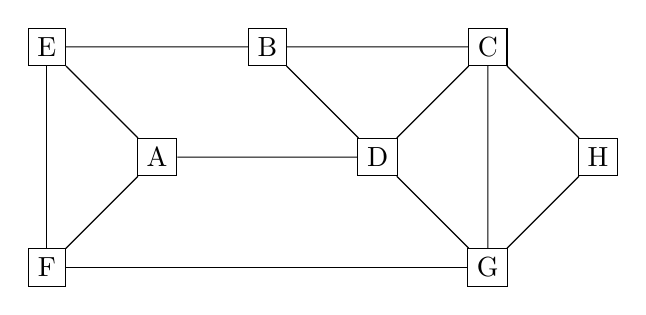
\begin{tikzpicture}[scale=1.4]
            \node[draw] (A) at (1,1) {A};
            \node[draw] (B) at (2,2) {B};
            \node[draw] (C) at (4,2) {C};
            \node[draw] (D) at (3,1) {D};
            \node[draw] (E) at (0,2) {E};
            \node[draw] (F) at (0,0) {F};
            \node[draw] (G) at (4,0) {G};
            \node[draw] (H) at (5,1) {H};

            \draw (A)--(F);
            \draw (A)--(E);
            \draw (E)--(F);
            \draw (A)--(D);
            \draw (E)--(B);
            \draw (F)--(G);
            \draw (D)--(B);
            \draw (B)--(C);
            \draw (D)--(C);
            \draw (D)--(G);
            \draw (G)--(C);
            \draw (G)--(H);
            \draw (H)--(C);
        \end{tikzpicture}
    \end{center}
    \begin{enumerate}
        \item On déploie le protocole RIP sur le réseau ci-dessus. Appliquer le protocole de Bellman-Ford pour déterminer les plus courts chemins partant du routeur A.
    \end{enumerate}
    \begin{center}
        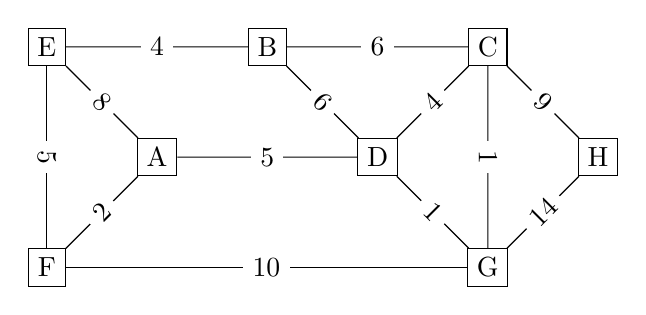
\begin{tikzpicture}[scale=1.4]
            \node[draw] (A) at (1,1) {A};
            \node[draw] (B) at (2,2) {B};
            \node[draw] (C) at (4,2) {C};
            \node[draw] (D) at (3,1) {D};
            \node[draw] (E) at (0,2) {E};
            \node[draw] (F) at (0,0) {F};
            \node[draw] (G) at (4,0) {G};
            \node[draw] (H) at (5,1) {H};

            \draw (A)--(F) node[sloped, midway, fill=white]{2};
            \draw (A)--(E) node[sloped, midway, fill=white]{8};
            \draw (E)--(F) node[sloped, midway, fill=white]{5};
            \draw (A)--(D) node[sloped, midway, fill=white]{5};
            \draw (E)--(B) node[sloped, midway, fill=white]{4};
            \draw (F)--(G) node[sloped, midway, fill=white]{10};
            \draw (D)--(B) node[sloped, midway, fill=white]{6};
            \draw (B)--(C) node[sloped, midway, fill=white]{6};
            \draw (D)--(C) node[sloped, midway, fill=white]{4};
            \draw (D)--(G) node[sloped, midway, fill=white]{1};
            \draw (G)--(C) node[sloped, midway, fill=white]{1};
            \draw (G)--(H) node[sloped, midway, fill=white]{14};
            \draw (H)--(C) node[sloped, midway, fill=white]{9};
        \end{tikzpicture}
    \end{center}
    \begin{enumerate}
        \setcounter{enumi}{1}
        \item     Le réseau est finalement plus complexe.
         Que représentent les pondérations indiquées si on applique le protocole RIP? OSPF?
    \end{enumerate} 
    En partant de A:
    \begin{enumerate}
        \setcounter{enumi}{2}
        \item Appliquer l'algorithme de Bellman-Ford sur le graphe.
        \item Appliquer l'algorithme de Dijkstra sur le graphe.
    \end{enumerate}
\end{exo}
\begin{exo}\textbf{Sujet 0 bac (retour)}\\
\begin{center}
\centering
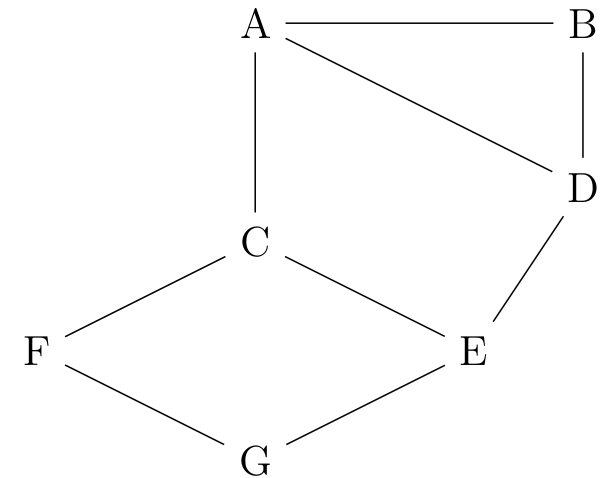
\includegraphics[width=4cm]{ressources/exo-bac.png}
\end{center}
\begin{enumerate}
    \item Appliquer l'algorithme de Bellman-Ford pour calculer les plus courts chemins depuis le routeur A.
    \item Comparer les résultats avec les tables de routage données dans les exercices \emph{RIP}.
\end{enumerate}
\begin{center}
    \centering
    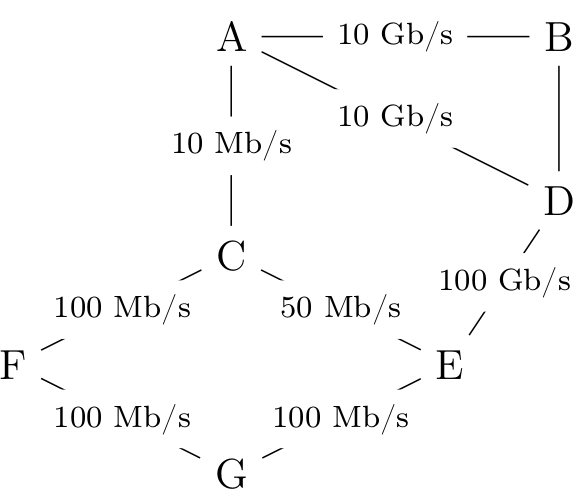
\includegraphics[width=4.5cm]{ressources/bacblanc.png}
    \end{center}
    \begin{enumerate}
        \setcounter{enumi}{2}
        \item Le réseau est en fait constitué de plusieurs technologies. Le coût de la liaison B-D est 5. Rappeler la valeur de la bande passante de ce réseau.
        \item Le protocole OSPF est appliqué pour calculer les routes. En appliquant l'algorithme de Dijkstra, calculer les plus courts chemins vers chaque routeur.
    \end{enumerate}
\end{exo}
\end{document}